% Assignment source: ne630/homework/markdown/HW05.md.
% No matching solutions existed for the six current problems.  Solutions are
% drafted from the archived Fall 2026 course notebook and earlier solution
% language identified in the comments below.

% --------------------------------------------------------------------------
% Problem 1
% --------------------------------------------------------------------------
\noindent{\bf Problem 1}.  Using the BNL NNDC Sigma interface, determine which
reactions a neutron can induce, based on the available cross sections, for
each of the following nuclides:
\begin{enumerate}[label=(\alph*)]
\item \isoA{H}{1}
\item \isoA{B}{10}
\item \isoA{U}{238}
\end{enumerate}

\begin{draftsolution}
The available reaction cross sections are:

\begin{enumerate}[label=(\alph*)]
\item For \isoA{H}{1}, the principal reactions are elastic scattering and
radiative capture:
\[
 \isoA{H}{1}(n,n)\isoA{H}{1}
 \qquad\text{and}\qquad
 \isoA{H}{1}(n,\gamma)\isoA{H}{2}.
\]

\item For \isoA{B}{10}, the course data include elastic scattering, inelastic
scattering, radiative capture, $(n,p)$, $(n,d)$, and $(n,\alpha)$.
Representative reactions are
\[
\begin{split}
 \isoA{B}{10}(n,\gamma)\isoA{B}{11},\qquad
 \isoA{B}{10}(n,p)\isoA{Be}{10},\\
 \isoA{B}{10}(n,d)\isoA{Be}{9},\qquad
 \isoA{B}{10}(n,\alpha)\isoA{Li}{7}.
\end{split}
\]
The \isoA{Li}{7} product is often born in an excited state, in which case its
subsequent de-excitation also produces a gamma ray.

\item For \isoA{U}{238}, the principal curves used in the course data are
elastic scattering, inelastic scattering, radiative capture, and fission:
\[
 \isoA{U}{238}(n,\gamma)\isoA{U}{239}
\]
together with \isoA{U}{238}$(n,n')$\isoA{U}{238}$^*$ and
\isoA{U}{238}$(n,f)$.  The full evaluated file also includes threshold
multiple-neutron reactions such as
\[
 \isoA{U}{238}(n,2n)\isoA{U}{237}
\]
once the incident neutron has sufficient energy.
\end{enumerate}

I would not count $\sigma_t$ as a separate interaction: the total cross
section is the sum of the available partial cross sections.  Similarly,
$\bar{\nu}$ is included in the nuclear data, but it is not a reaction cross
section.

\medskip
\noindent\emph{Data note:} The reaction inventory above follows the archived
BNL SIGMA/ENDF data used to prepare the course notebook.  The full ENDF file
contains more detailed threshold channels than the reduced course data, and
the way those channels are grouped can depend on the retrieval selected in
SIGMA.
\end{draftsolution}

\newpage

% --------------------------------------------------------------------------
% Problem 2
% Figure is the embedded output of ne630/notebooks/lesson_05.ipynb, cell 8.
% --------------------------------------------------------------------------
\noindent{\bf Problem 2}.  Sketch $\sigma_e$ and $\sigma_\gamma$ for
\isoA{H}{1} over $10^{-3}<E<10^7~\mathrm{eV}$.  Use log--log axes, with
$10^{-4}<\sigma<10^4~\mathrm{b}$ on the vertical axis.  Here, the subscript
$e$ denotes elastic scattering.

\begin{draftsolution}
The two cross sections are shown below.

\begin{center}
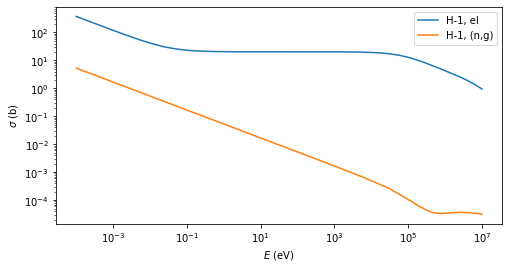
\includegraphics[width=0.82\textwidth]{figures/hw05_h1_cross_sections.png}
\end{center}

The elastic-scattering cross section is nearly constant at about 20~b over a
large part of the low- and intermediate-energy range, and then decreases in
the fast range.  In contrast, the radiative-capture cross section decreases
approximately as $1/v$ over the low-energy range.  Because
$v\propto\sqrt{E}$,
\[
 \sigma_\gamma(E)\propto\frac{1}{v}\propto E^{-1/2}.
\]
Thus, the capture curve is approximately a straight line with slope $-1/2$
on the log--log plot.  The evaluated curve departs from a perfect $1/v$ law
at higher energies.

For reference, the values extracted below are
\[
\begin{array}{c|cc}
 &1~\mathrm{eV}&1~\mathrm{MeV}\\
\hline
\sigma_e&20.5933~\mathrm{b}&4.28306~\mathrm{b}\\
\sigma_\gamma&5.31149\times10^{-2}~\mathrm{b}
              &3.38313\times10^{-5}~\mathrm{b}.
\end{array}
\]

\noindent\emph{Data note:} The plotted curves and quoted values are from the
archived BNL SIGMA/ENDF evaluation used in the Fall 2026 course notebook.  A
fresh export from another evaluated library or processing temperature may
differ slightly.
\end{draftsolution}

\newpage

% --------------------------------------------------------------------------
% Problem 3
% Numerical work follows ne630/notebooks/lesson_05.ipynb, cells 11--12.
% --------------------------------------------------------------------------
\noindent{\bf Problem 3}.  Using \textbf{Evaluated Data} in the Sigma
interface, extract the following cross sections at $1~\mathrm{eV}$ and
$1~\mathrm{MeV}$.  Use linear interpolation as needed.

\begin{center}
\begin{tabular}{|l|c|c|}
\hline
Quantity for \isoA{H}{1}&$1~\mathrm{eV}$&$1~\mathrm{MeV}$\\
\hline
$\sigma_e~(\mathrm{b})$&&\\
$\sigma_\gamma~(\mathrm{b})$&&\\
$\sigma_t~(\mathrm{b})$&&\\
\hline
\end{tabular}
\end{center}

\noindent\emph{Interpolation note:} Given $(x_1,y_1)$ and $(x_2,y_2)$,
evaluate $y$ at $x$, where $x_1<x<x_2$, using
\[
 y(x)=\frac{(x-x_1)y_2+(x_2-x)y_1}{x_2-x_1}.
\]
\textbf{Hint:} Based on the available reactions, do you need to look up
$\sigma_t$, or can you construct it from the partial cross sections?

\begin{draftsolution}
Using the interpolation expression in the problem statement, the
elastic-scattering cross section at 1~eV is
\[
\begin{split}
 \sigma_e(1~\mathrm{eV})
 &=\frac{(1-0.40461)(20.2988)+(1.68858-1)(20.848)}
         {1.68858-0.40461}\\
 &\approx20.5933~\mathrm{b}.
\end{split}
\]
Similarly,
\[
\begin{split}
 \sigma_\gamma(1~\mathrm{eV})
 &=\frac{(1-0.826569)(0.0509196)+(1.07619-1)(0.0581121)}
         {1.07619-0.826569}\\
 &\approx0.0531149~\mathrm{b}.
\end{split}
\]

At 1~MeV, the corresponding interpolations give
\[
\begin{split}
 \sigma_e(1~\mathrm{MeV})
 &=\frac{(10^6-850000)(4.0527)+(1097760-10^6)(4.63652)}
         {1097760-850000}\\
 &\approx4.28306~\mathrm{b},\\[4pt]
 \sigma_\gamma(1~\mathrm{MeV})
 &=\frac{(10^6-800000)(3.67662\times10^{-5})
       +(2000000-10^6)(3.32443\times10^{-5})}
         {2000000-800000}\\
 &\approx3.38313\times10^{-5}~\mathrm{b}.
\end{split}
\]

At these two energies, the available interactions for \isoA{H}{1} are
elastic scattering and radiative capture.  Hence,
\[
 \sigma_t=\sigma_e+\sigma_\gamma.
\]
The completed table is
\begin{center}
\begin{tabular}{|l|r|r|}
\hline
Quantity for \isoA{H}{1}&$1~\mathrm{eV}$&$1~\mathrm{MeV}$\\
\hline
$\sigma_e~(\mathrm{b})$&20.5933&4.28306\\
$\sigma_\gamma~(\mathrm{b})$&0.0531149&$3.38313\times10^{-5}$\\
$\sigma_t~(\mathrm{b})$&20.6464&4.28309\\
\hline
\end{tabular}
\end{center}

\noindent\emph{Data note:} These numbers use the interpolation points stored
in the archived course notebook.  Their last quoted digits are evaluation-
and interpolation-dependent.
\end{draftsolution}

\newpage
% --------------------------------------------------------------------------
% Problem 4
% Figure is the embedded output of ne630/notebooks/lesson_05.ipynb, cell 15.
% --------------------------------------------------------------------------
\noindent{\bf Problem 4}.  Determine which interaction $X$ dominates the
total cross section of \isoA{B}{10}.  How does $\sigma_X(E)$ depend on $E$?

\noindent\textbf{Hint:} Straight lines on log--log plots indicate power laws
of the form $y(x)=x^p$.

\begin{draftsolution}
The available partial cross sections are shown below.

\begin{center}
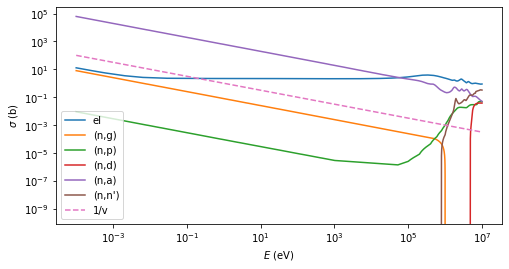
\includegraphics[width=0.82\textwidth]{figures/hw05_b10_cross_sections.png}
\end{center}

The dominant low-energy interaction is
\[
 \isoA{B}{10}(n,\alpha)\isoA{Li}{7}.
\]
Away from the higher-energy structure, the $(n,\alpha)$ cross section is
approximately a $1/v$ cross section:
\[
 \boxed{\sigma_\alpha(E)\propto\frac{1}{v}\propto E^{-1/2}}.
\]
This appears as a straight line with slope $-1/2$ on a log--log plot.

At fast-neutron energies, elastic and inelastic scattering become comparable
to, and eventually larger than, the $(n,\alpha)$ cross section.  Thus,
``dominant'' here refers to the broad low-energy range for which \isoA{B}{10}
is normally used as a neutron absorber; it does not mean that $(n,\alpha)$ is
the largest partial cross section at every energy shown.
\end{draftsolution}

\newpage

% --------------------------------------------------------------------------
% Problem 5
% Values follow ne630/notebooks/lesson_05.ipynb and
% ne630_problems/lesson_05/HW05_solution_work.ipynb.
% --------------------------------------------------------------------------
\noindent{\bf Problem 5}.  Using the Sigma interface, determine the missing
values in the following table.  All cross sections are in barns.

\begin{center}
\begin{tabular}{|l|l|c|c|}
\hline
Nuclide&Quantity&$1~\mathrm{eV}$&$1~\mathrm{MeV}$\\
\hline
\isoA{U}{235}&$\sigma_t$&&\\
\isoA{U}{235}&$\sigma_e$&&\\
\isoA{U}{235}&$\sigma_\gamma$&&\\
\isoA{U}{235}&$\sigma_f$&&\\
\isoA{U}{235}&$\bar\nu$&&\\
\isoA{U}{238}&$\sigma_t$&&\\
\isoA{U}{238}&$\sigma_e$&&\\
\isoA{U}{238}&$\sigma_\gamma$&&\\
\isoA{U}{238}&$\sigma_f$&&\\
\isoA{U}{238}&$\bar\nu$&&\\
\hline
\end{tabular}
\end{center}

\begin{draftsolution}
Here, I'm using the actual text files from BNL Sigma, so these numbers ought
to be the same that you get by hand/calculator.

\begin{center}
\begin{tabular}{|l|l|r|r|}
\hline
Nuclide&Quantity&$1~\mathrm{eV}$&$1~\mathrm{MeV}$\\
\hline
\isoA{U}{235}&$\sigma_t~(\mathrm{b})$&91.60&6.85619\\
\isoA{U}{235}&$\sigma_e~(\mathrm{b})$&13.14&3.65029\\
\isoA{U}{235}&$\sigma_\gamma~(\mathrm{b})$&10.40&0.108433\\
\isoA{U}{235}&$\sigma_f~(\mathrm{b})$&67.77&1.19979\\
\isoA{U}{235}&$\bar\nu$&2.421&2.51601\\
\hline
\isoA{U}{238}&$\sigma_t~(\mathrm{b})$&9.687&7.12538\\
\isoA{U}{238}&$\sigma_e~(\mathrm{b})$&9.085&4.72403\\
\isoA{U}{238}&$\sigma_\gamma~(\mathrm{b})$&0.5105&0.128299\\
\isoA{U}{238}&$\sigma_f~(\mathrm{b})$&$2.963\times10^{-6}$&0.0135521\\
\isoA{U}{238}&$\bar\nu$&2.492&2.56336\\
\hline
\end{tabular}
\end{center}

The small \isoA{U}{238} fission cross section at 1~eV is not a typo.
Fission of \isoA{U}{238} is possible at low energies in the evaluated data,
but it is extremely improbable.  Its fission cross section increases
substantially in the fast range, which is why \isoA{U}{238} is normally
described as a threshold-fission nuclide.

\medskip
\noindent\emph{Data note:} The 1-eV values are retained as rounded constants
in the Fall 2026 course notebook; the raw SIGMA text files are not present in
the repository.  The 1-MeV values are preserved at greater precision in the
archived solution notebook.  These are values from that archived evaluation,
not library-independent constants.
\end{draftsolution}

\newpage

% --------------------------------------------------------------------------
% Problem 6
% Opening/process language follows the style of the original lesson_05
% solution; numerical work follows ne630/notebooks/lesson_05.ipynb,
% cells 19--29. No matching solution exists for the current problem.
% --------------------------------------------------------------------------
\noindent{\bf Problem 6}.  Our TRIGA fuel consists of a mixture of zirconium
hydride ($\mathrm{ZrH}_{1.6}$) and uranium metal with a bulk mass density of
$7.1~\mathrm{g\,cm^{-3}}$.
\begin{itemize}
\item Uranium makes up 8.5\% of the mixture \textbf{by mass}.
\item The uranium is enriched to 20\% \isoA{U}{235} \textbf{by atom}; assume
the balance is \isoA{U}{238}.
\item Natural zirconium consists of \isoA{Zr}{90} (51.5\%), \isoA{Zr}{91}
(11.2\%), \isoA{Zr}{92} (17.1\%), \isoA{Zr}{94} (17.4\%), and \isoA{Zr}{96}
(2.8\%), all by atom.
\item Assume that \isoA{H}{1}, \isoA{U}{235}, and \isoA{U}{238} are the only
other nuclides.
\end{itemize}
Use $N_A=6.022\times10^{23}~\mathrm{mol^{-1}}$ and approximate each isotope's
molar mass by its mass number in $\mathrm{g\,mol^{-1}}$.

\begin{enumerate}[label=(\alph*)]
\item Compute the indicated molecular and atomic number densities.  The
following expressions provide a starting point:
\[
\begin{gathered}
\overline M_{\mathrm{Zr}}
=0.515(90)+0.112(91)+0.171(92)+0.174(94)+0.028(96),\\
M_{\mathrm{ZrH}_{1.6}}=\overline M_{\mathrm{Zr}}+1.6(1),\qquad
n_{\mathrm{ZrH}_{1.6}}
=\frac{(0.915)(7.1)N_A}{M_{\mathrm{ZrH}_{1.6}}},\\
n_{\isoA{H}{1}}=1.6n_{\mathrm{ZrH}_{1.6}},\qquad
n_{\isoA{Zr}{90}}=0.515n_{\mathrm{ZrH}_{1.6}},\\[2pt]
\overline M_{\mathrm U}=0.20(235)+0.80(238),\qquad
n_{\mathrm U}=\frac{(0.085)(7.1)N_A}{\overline M_{\mathrm U}},\\
n_{\isoA{U}{235}}=0.20n_{\mathrm U},\qquad
n_{\isoA{U}{238}}=0.80n_{\mathrm U}.
\end{gathered}
\]
Report all six requested densities: $n_{\mathrm{ZrH}_{1.6}}$,
$n_{\isoA{H}{1}}$, $n_{\isoA{Zr}{90}}$, $n_{\mathrm U}$,
$n_{\isoA{U}{235}}$, and $n_{\isoA{U}{238}}$.
\item Suppose the elastic-scattering cross section for zirconium, averaged
over its naturally occurring isotopes, is $6~\mathrm b$ at all neutron
energies and that all other interactions with zirconium are negligible.
Using the cross sections collected above, compute the macroscopic total,
elastic-scattering, and absorption cross sections of the fuel at $1~\mathrm{eV}$.
\item If a $1~\mathrm{eV}$ neutron interacts in the fuel, what is the
probability that the interaction is an elastic collision?
\item If a $1~\mathrm{eV}$ neutron has an elastic collision, what is the
probability that it collides with \isoA{H}{1}?
\item On average, how far does a $1~\mathrm{eV}$ neutron travel in this fuel
before undergoing any interaction?
\item If a $1~\mathrm{eV}$ neutron is absorbed, what is the probability that
it induces fission?
\item If a $1~\mathrm{eV}$ neutron induces fission, what is the expected
number of emitted neutrons?  Account for both uranium isotopes by using a
fission-rate-weighted value of $\bar\nu$.
\end{enumerate}

\begin{draftsolution}
To answer (a)--(g), we need to compute the number density of each nuclide in
the fuel mixture and to evaluate macroscopic cross sections for each nuclide
and reaction.  Given the tabular data and repeated calculations, it is far
more convenient to use a short script (in, e.g., Python) or a spreadsheet than
to do each calculation by hand.  Here, I'm using Python to do the computations.

\begin{enumerate}[label=(\alph*)]
\item First, I'll compute the number densities given the mass density,
chemical formula, and uranium enrichment.  The average molar mass of natural
zirconium is
\[
\begin{split}
 \overline M_{\mathrm{Zr}}
 &=0.515(90)+0.112(91)+0.171(92)+0.174(94)+0.028(96)\\
 &=91.318~\mathrm{g/mol}.
\end{split}
\]
Therefore,
\[
 M_{\mathrm{ZrH}_{1.6}}=91.318+1.6(1)=92.918~\mathrm{g/mol}.
\]
The zirconium-hydride portion of the fuel has an effective mass density
$(1-0.085)(7.1)=6.4965~\mathrm{g/cm^3}$, and hence
\[
\begin{split}
 n_{\mathrm{ZrH}_{1.6}}
 &=\frac{(0.915)(7.1)(6.022\times10^{23})}{92.918}\\
 &=4.21037\times10^{22}~\mathrm{cm^{-3}}.
\end{split}
\]
There is one zirconium atom and 1.6 hydrogen atoms per formula unit, so
\[
\begin{split}
 n_{\isoA{H}{1}}&=1.6n_{\mathrm{ZrH}_{1.6}}
 =6.73659\times10^{22}~\mathrm{cm^{-3}},\\
 n_{\isoA{Zr}{90}}&=0.515n_{\mathrm{ZrH}_{1.6}}
 =2.16834\times10^{22}~\mathrm{cm^{-3}}.
\end{split}
\]
For the uranium,
\[
 \overline M_{\mathrm U}=0.20(235)+0.80(238)=237.4~\mathrm{g/mol},
\]
so that
\[
\begin{split}
 n_{\mathrm U}
 &=\frac{(0.085)(7.1)(6.022\times10^{23})}{237.4}
 =1.53087\times10^{21}~\mathrm{cm^{-3}},\\
 n_{\isoA{U}{235}}&=0.20n_{\mathrm U}
 =3.06173\times10^{20}~\mathrm{cm^{-3}},\\
 n_{\isoA{U}{238}}&=0.80n_{\mathrm U}
 =1.22469\times10^{21}~\mathrm{cm^{-3}}.
\end{split}
\]
Thus, all six requested densities are
\begin{center}
\begin{tabular}{|l|r|r|}
\hline
Quantity&$\mathrm{cm^{-3}}$&$\mathrm{(b\,cm)^{-1}}$\\
\hline
$n_{\mathrm{ZrH}_{1.6}}$&$4.21037\times10^{22}$&0.0421037\\
$n_{\isoA{H}{1}}$&$6.73659\times10^{22}$&0.0673659\\
$n_{\isoA{Zr}{90}}$&$2.16834\times10^{22}$&0.0216834\\
$n_{\mathrm U}$&$1.53087\times10^{21}$&0.00153087\\
$n_{\isoA{U}{235}}$&$3.06173\times10^{20}$&0.000306173\\
$n_{\isoA{U}{238}}$&$1.22469\times10^{21}$&0.00122469\\
\hline
\end{tabular}
\end{center}
For the individual nuclides, I've adopted the useful unit of a/b-cm.  This
unit builds in the factor of $10^{-24}~\mathrm{cm^2/b}$ so that $\Sigma$'s
can be computed directly.

\item Then, I compute the individual nuclide-reaction, macroscopic cross
sections.  Using the 1-eV values from Problem 5, the hydrogen values from
Problem 3, and $\sigma_e^{\mathrm{Zr}}=6~\mathrm b$ gives
\[
\begin{split}
 \Sigma_e=10^{-24}\big[&n_{\isoA{U}{235}}(13.14)
 +n_{\isoA{U}{238}}(9.085)+n_{\mathrm{ZrH}_{1.6}}(6)\\
 &+n_{\isoA{H}{1}}(20.5933)\big]
 \approx\boxed{1.65506~\mathrm{cm^{-1}}},
\end{split}
\]
and
\[
\begin{split}
 \Sigma_a=10^{-24}\big[&n_{\isoA{U}{235}}(10.40+67.77)
 +n_{\isoA{U}{238}}(0.5105+2.963\times10^{-6})\\
 &+n_{\isoA{H}{1}}(0.0531149)\big]
 \approx\boxed{0.0281369~\mathrm{cm^{-1}}}.
\end{split}
\]
Using the tabulated total cross sections,
\[
\begin{split}
 \Sigma_t=10^{-24}\big[&n_{\isoA{U}{235}}(91.60)
 +n_{\isoA{U}{238}}(9.687)+n_{\mathrm{ZrH}_{1.6}}(6)\\
 &+n_{\isoA{H}{1}}(20.6464)\big]
 \approx\boxed{1.68340~\mathrm{cm^{-1}}}.
\end{split}
\]
The small difference between $\Sigma_t$ and $\Sigma_e+\Sigma_a$ is due to
the precision retained in the archived, separately interpolated microscopic
cross sections and any small channels not listed individually.

\item If a neutron interacts, the probability that the interaction is an
elastic collision is
\[
 P(e\mid t)=\frac{R_e}{R_t}=\frac{\Sigma_e\phi}{\Sigma_t\phi}
 =\frac{\Sigma_e}{\Sigma_t}
 =\frac{1.65506}{1.68340}\approx\boxed{0.9832}.
\]

\item The macroscopic elastic-scattering cross section of hydrogen alone is
\[
 \Sigma_e^{\isoA{H}{1}}=n_{\isoA{H}{1}}\sigma_e^{\isoA{H}{1}}
 \approx1.38729~\mathrm{cm^{-1}}.
\]
Therefore, given that an elastic collision occurred,
\[
 P(\isoA{H}{1}\mid e)=\frac{\Sigma_e^{\isoA{H}{1}}}{\Sigma_e}
 =\frac{1.38729}{1.65506}\approx\boxed{0.8382}.
\]

\item The average distance to any interaction is the mean free path:
\[
 \lambda=\frac{1}{\Sigma_t}=\frac{1}{1.68340}
 \approx\boxed{0.5940~\mathrm{cm}}.
\]

\item The macroscopic fission cross section is
\[
\begin{split}
 \Sigma_f=10^{-24}\big[n_{\isoA{U}{235}}(67.77)
 +n_{\isoA{U}{238}}(2.963\times10^{-6})\big]
 =0.0207494~\mathrm{cm^{-1}}.
\end{split}
\]
Consequently, given that an absorption occurred,
\[
 P(f\mid a)=\frac{\Sigma_f}{\Sigma_a}
 =\frac{0.0207494}{0.0281369}\approx\boxed{0.7374}.
\]

\item Finally, the fission-rate-weighted neutron yield is
\[
 \overline\nu=
 \frac{\overline\nu_{\isoA{U}{235}}\Sigma_f^{\isoA{U}{235}}
       +\overline\nu_{\isoA{U}{238}}\Sigma_f^{\isoA{U}{238}}}
      {\Sigma_f^{\isoA{U}{235}}+\Sigma_f^{\isoA{U}{238}}}.
\]
Using
\[
 \Sigma_f^{\isoA{U}{235}}=0.020749364~\mathrm{cm^{-1}},\qquad
 \Sigma_f^{\isoA{U}{238}}=3.62877\times10^{-9}~\mathrm{cm^{-1}},
\]
and $\overline\nu_{\isoA{U}{235}}=2.421$ and
$\overline\nu_{\isoA{U}{238}}=2.492$ gives
\[
 \boxed{\overline\nu\approx2.421\text{ neutrons per fission}}.
\]
The \isoA{U}{238} contribution is negligible at 1~eV, so the result is
effectively the \isoA{U}{235} value.
\end{enumerate}

\noindent\emph{Data note:} Parts (b)--(g) inherit the rounded, archived BNL
SIGMA/ENDF values used in Problems 3 and 5.  The displayed arithmetic is
internally consistent with those values, but the extra digits should not be
interpreted as physical accuracy.
\end{draftsolution}

\clearpage
